%report on transformation; reflection, rotation, scaling, translation
\documentclass[12pt]{article}

\usepackage{amsmath}
\usepackage{graphicx}
\usepackage[a4paper]{geometry}

\geometry{
  textwidth=\dimexpr\paperwidth-29mm,
  textheight=\dimexpr\paperheight-32mm,
  noheadfoot,
  nomarginpar
}

\setlength{\topskip}{0mm}
\setlength{\parindent}{0mm}

\title{Transformation of a given shape}
\date{}
\author{}

\begin{document}
	\maketitle
	\vspace{-2cm}

	\section{Objective}
	To transform a given shape using the following transformations:
	\begin{itemize}
		\item Reflection
		\item Rotation
		\item Translation
	\end{itemize}
	
	\section{Theory}
	\subsection{Reflection}
	Reflection is a transformation that produces a mirror image of an object. The mirror image is generated by reflecting the object across an axis. The axis is called the line of reflection.
	In two dimensions, the line of reflection is a line in a plane and is perpendicular to the line containing the points and its image.
	Mathematically, the reflection of a point $(x,y)$ across the x-axis is $(x,-y)$ and the reflection across the y-axis is $(-x,y)$.

	\subsection{Rotation}
	Rotation is a transformation that turns a figure about a fixed point called the center of rotation. An object and its rotation are the same shape and size, but the figures may be turned in different directions.
	Mathematically, the rotation of a point $(x,y)$ about the origin through an angle $\theta$ in the counter-clockwise direction is given by:
	\[(x\cos\theta - y\sin\theta, x\sin\theta + y\cos\theta)\]
	A more general form of rotation is about a point $(x_{r}, y_{r})$, which is given by:
	\[(x_{r} + (x - x_{r})\cos\theta - (y - y_{r})\sin\theta, y_{r} + (x - x_{r})\sin\theta + (y - y_{r})\cos\theta)\]
	The above formulaes support rotation in both the clockwise and counter-clockwise direction. For clockwise rotation, the angle $\theta$ is negative.
	An even more general approach to rotate coordinates is by using the following rotation matrix. Objects can also be rotated by an angle theta about an axis $(x_{r}, y_{r})$ using the rotation matrix:
	\begin{equation*}
		\begin{bmatrix}
			\cos\theta & -\sin\theta & x_{r}(1 - \cos\theta) + y_{r}\sin\theta \\
			\sin\theta & \cos\theta & y_{r}(1 - \cos\theta) - x_{r}\sin\theta \\
			0 & 0 & 1
		\end{bmatrix}
		\begin{bmatrix}
			x \\
			y \\
			1
		\end{bmatrix}
		=	
		\begin{bmatrix}
			x_{r} + (x - x_{r})\cos\theta - (y - y_{r})\sin\theta \\
			y_{r} + (x - x_{r})\sin\theta + (y - y_{r})\cos\theta \\
			1
		\end{bmatrix}
	\end{equation*}

	\subsection{Translation}
	Translation is a transformation that moves a figure in a straight line without turning it or making it bigger or smaller.
	Mathematically, the translation of a point $(x,y)$ by a vector $(a,b)$ is given by $(x+a,y+b)$.

	\section{Algorithm}
	\subsection{Reflection}
	\begin{enumerate}
		\item Start
		\item Read the coordinates of the vertices of the shape
		\item Read the axis of reflection
		\item If the axis of reflection is x-axis, then
		\begin{enumerate}
			\item For each vertex, negate the y-coordinate
		\end{enumerate}
		\item Else if the axis of reflection is y-axis, then
		\begin{enumerate}
			\item For each vertex, negate the x-coordinate
		\end{enumerate}
		\item Else
		\begin{enumerate}
			\item For each vertex, negate both the x and y coordinates
		\end{enumerate}
		\item Print the coordinates of the new vertices or draw the reflected shape
		\item Stop
	\end{enumerate}

	\subsection{Rotation}
	\begin{enumerate}
		\item Start
		\item Read the coordinates of the vertices of the shape
		\item Read the angle of rotation
		\item Read the center of rotation
		\item For each vertex, rotate it about the center of rotation by the angle of rotation using the rotation matrix
		\item Print the coordinates of the vertices of the rotated shape or display the new shape.
		\item Stop
	\end{enumerate}

	\subsection{Translation}
	\begin{enumerate}
		\item Start
		\item Read the coordinates of the vertices of the shape
		\item Read the vector of translation
		\item For each vertex, do
		\begin{enumerate}
			\item Add the vector of translation to the coordinates of the vertex
		\end{enumerate}
		\item Print the coordinates of the new vertices or display the translated shape
		\item Stop
	\end{enumerate}

\newpage
	\section{Source Code}

\begin{verbatim}
#include <stdio.h>
#include <math.h>
#include <graphics.h>

#define width 640
#define height 480

#define PI 3.1415926535889

void axes()
{
    // print axes
    line(width / 2, 0, width / 2, height);
    line(0, height / 2, width, height / 2);
}

void translate(unsigned* x, unsigned* y)
{
    // translates the coordinates to the new axes
    *x = (*x + width / 2) % width;
    *y = (-*y + height / 2) % height;
}

void drawTriangle(unsigned coordinates[3][2])
{
    // draw functions guarantee that the data received is not modified
    // so work with a copy of the coordinates; it's a pointer
    unsigned copy[3][2];
    for (unsigned i = 0; i < 3; i++)
    {
        copy[i][0] = coordinates[i][0];
        copy[i][1] = coordinates[i][1];
    }
    // only needs to be done here; translate to the axes defined by the computer
    for (unsigned i = 0; i < 3; i++) translate(&copy[i][0], &copy[i][1]);
    // plot the translated points
    for (unsigned i = 0; i < 3; i++)
        line(copy[i][0], copy[i][1], copy[(i + 1) % 3][0], copy[(i + 1) % 3][1]);
}

void reflectXaxis(unsigned num_points, unsigned coordinates[][2])
{
    // make the y coordinates negative
    for (unsigned i = 0; i < num_points; i++) coordinates[i][1] = -coordinates[i][1];
}

void reflectYaxis(unsigned num_points, unsigned coordinates[][2])
{
    // make the x coordinates negative
    for (unsigned i = 0; i < num_points; i++) coordinates[i][0] = -coordinates[i][0];
}

void rotate(unsigned num_points, unsigned coordinates[][2], float theta, unsigned axis[2])
{
    // buffer the coordinates because the updates are simultaneous
    unsigned copy[2];

    // rotate the coordinates by theta degrees
    for (unsigned i = 0; i < num_points; i++)
    {
        copy[0] = axis[0] + (coordinates[i][0] - axis[0]) * cos(theta * PI / 180)
                - (coordinates[i][1] - axis[1]) * sin(theta * PI / 180);
        copy[1] = axis[1] + (coordinates[i][0] - axis[0]) * sin(theta * PI / 180)
                + (coordinates[i][1] - axis[1]) * cos(theta * PI / 180);

        // copy the rotated coordinates back to the original array
        coordinates[i][0] = copy[0];
        coordinates[i][1] = copy[1];
    }
}

int main()
{
    int gd = DETECT, gm;
    initgraph(&gd, &gm, "");
    setcolor(GREEN);

    axes();
    // coordinates of a triangle in the first quadrant
    unsigned triangle[3][2] =
    {
        {50, 50},
        {50, 200},
        {200, 50}
    };
    // draw the triangle in the first quadrant 
    drawTriangle(triangle);

    // REFLECTION stuff reflect the triangle with respect to the x-axis
    reflectXaxis(3, triangle);
    drawTriangle(triangle);
    // reflect the above triangle with respect to the y-axis
    reflectYaxis(3, triangle);
    drawTriangle(triangle);

    // reflect the above triangle with respect to the x-axis
    reflectXaxis(3, triangle);
    drawTriangle(triangle);

    // reflect once again to get the original triangle
    reflectYaxis(3, triangle);
    setcolor(RED);
    drawTriangle(triangle);

    // ROTATION stuff
    setcolor(BLUE);
    unsigned axis[2] = { 50, 50 };
    printf("%u %u\n", axis[0], axis[1]);
    float theta = -60.f;
    rotate(3, triangle, theta, axis);
    drawTriangle(triangle);

    getch();
    closegraph();
    return 0;
}
\end{verbatim}
	\section{Output}

	\begin{figure}[!h]
		\hspace*{-1cm}
		\centering
		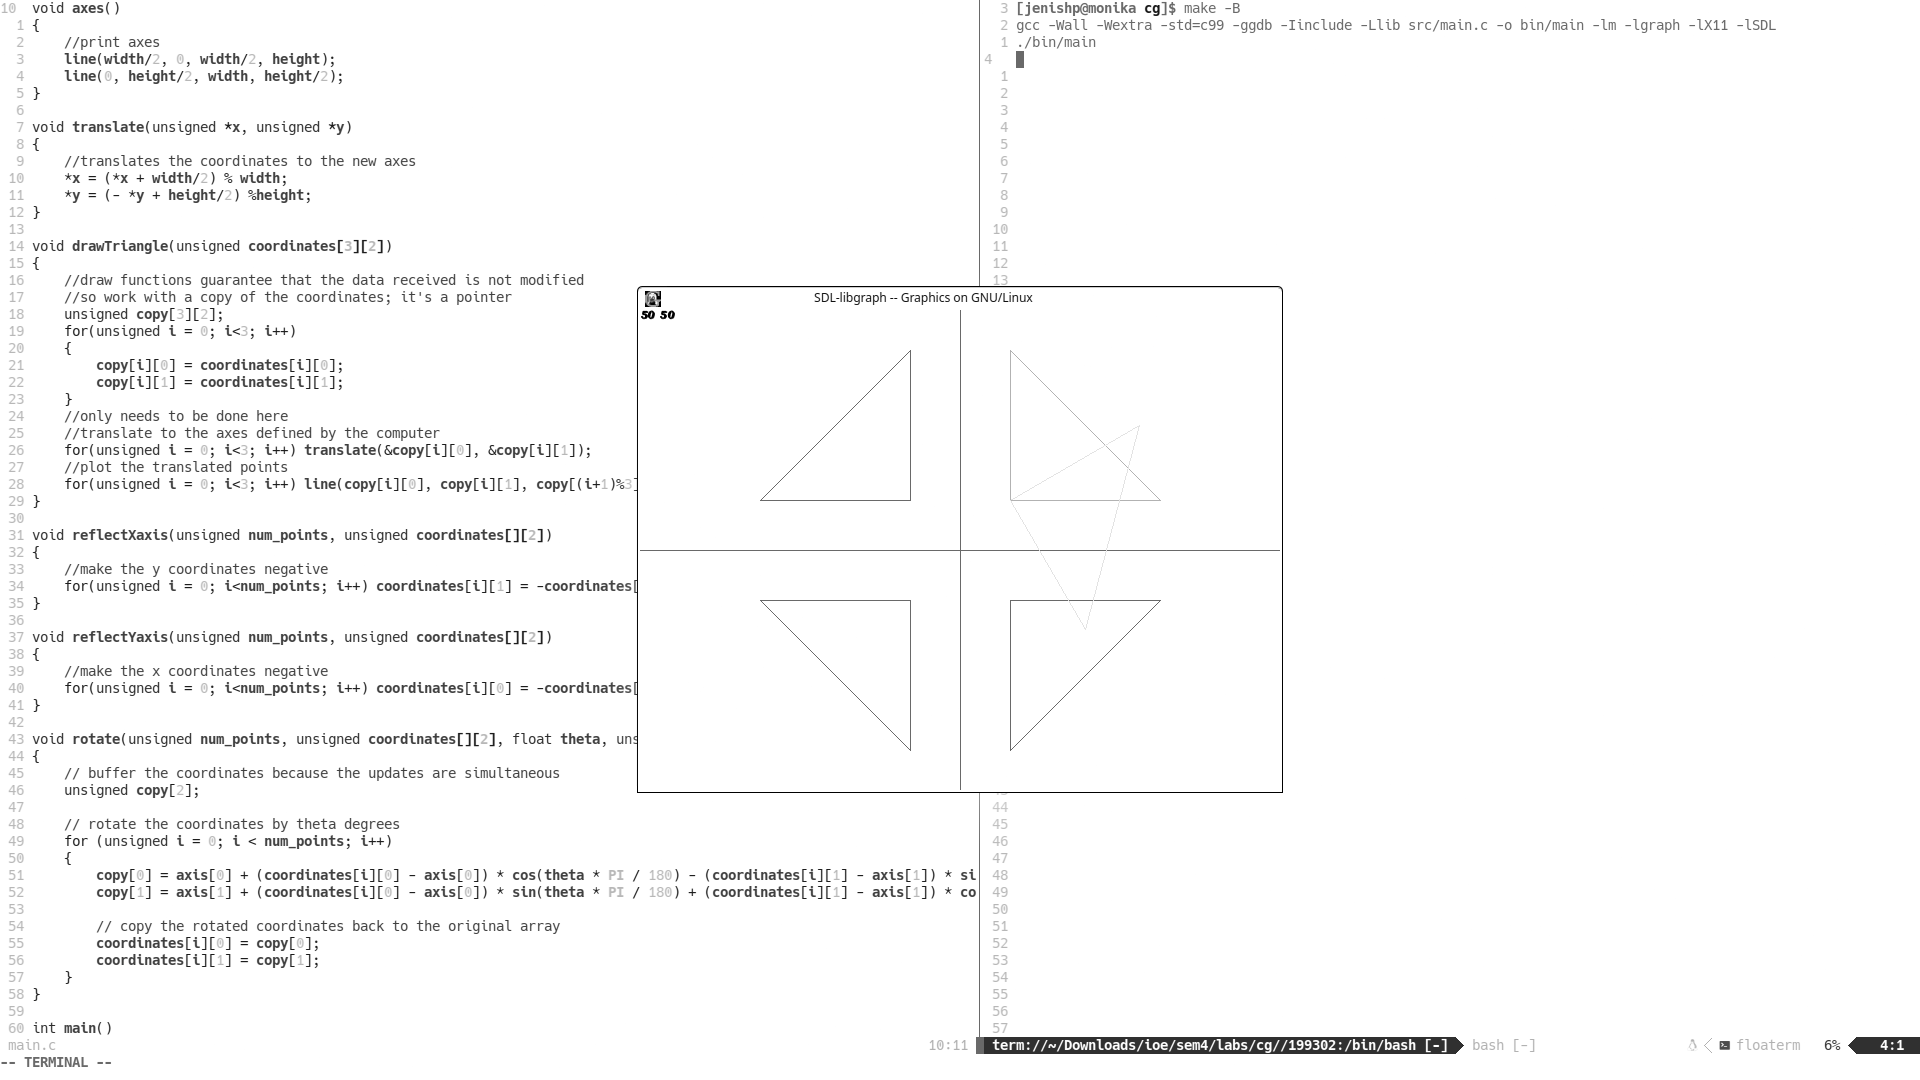
\includegraphics[width=1.01\linewidth]{output4.png}
		\caption{}
		\label{fig:}
	\end{figure}

	\section{Conclusion}
	Here, we have seen how to transform a given shape using the Reflection, Rotation and Translation.
	On transforming the shape, we can see that the shape is reflected about the x-axis, y-axis and to the 3rd quadrant.
	The shape is also rotated about the origin by an angle of 60 degrees in the clockwise direction about its vertex.
	To make the transformations easier, we have used a translation function to translate the coordinates to the axes defined by the computer just 
	before plotting the points. This virtually shifts the origin to the center of the screen and makes the transformations easier to understand.

\end{document}


